% Mini Research Problem - Artificial Intelligence (Advanced Topics in AI & ML)
% Compile:  pdflatex mrp.tex   (twice)
\documentclass[11pt,aspectratio=169]{beamer}

\usepackage[T1]{fontenc}
\usepackage{lmodern}
\usepackage{booktabs}
\usepackage{graphicx}
\usepackage{hyperref}
\hypersetup{hidelinks}

\usetheme{default}
\usecolortheme{dove}
\setbeamertemplate{navigation symbols}{}
\setbeamertemplate{itemize items}[circle]
\definecolor{accent}{HTML}{1B4F72}
\setbeamercolor{frametitle}{fg=accent}
\setbeamercolor{structure}{fg=accent}
\setbeamerfont{frametitle}{series=\bfseries,size=\large}
\setbeamerfont{footline}{size=\tiny}
\setbeamertemplate{footline}{%
  \hfill\usebeamerfont{footline}\color{gray}%
  \insertframenumber/\inserttotalframenumber\hspace{2ex}\vspace{1ex}}

\newcommand{\f}[1]{{\small\texttt{#1}}}
\newcommand{\link}[2]{\href{#1}{\color{accent}\underline{#2}}}
\newcommand{\repo}{https://github.com/Wangzx9908/ai-hw-SUMMER-2026-MRP}

\title{\bfseries Explainable AI for Network Intrusion Detection}
\subtitle{Using SHAP to understand why an ML-based IDS blocks a flow}
\author{Mini Research Problem \\ Artificial Intelligence -- Advanced Topics in AI \& ML}
\date{}

\begin{document}

{\setbeamertemplate{footline}{}
\begin{frame}[plain]
  \titlepage
  \vspace{-1.5em}
  \centering\small Code: \link{\repo}{github.com/Wangzx9908/ai-hw-SUMMER-2026-MRP}
\end{frame}}

% ---------------------------------------------------------------- tl;dr
\begin{frame}{tl;dr}
\small
\begin{block}{Motivation}
An ML-based intrusion detection system only outputs \emph{normal} or
\emph{attack}. A network engineer cannot act on that: was the flow blocked
because of abnormal TCP flags, or because the payload was empty? Without a
reason, nobody trusts the system enough to let it drop real traffic.
\end{block}
\begin{block}{Main idea}
Train a Random Forest on the NSL-KDD flow dataset to classify traffic into
\f{normal / DoS / Probe / R2L / U2R}, then apply \textbf{SHAP} to see which of
the 41 flow features drove each decision -- globally (per attack type) and
locally (a single flow).
\end{block}
\begin{block}{Results}
\begin{itemize}\itemsep1pt
  \item 74.3\,\% accuracy on the official test set (DoS recall 77\,\%, Probe 65\,\%).
  \item SHAP shows the model relies on exactly the features a network engineer
        would use: DoS $\to$ \f{serror\_rate}, \f{count}; Probe $\to$ \f{src\_bytes}=0,
        \f{diff\_srv\_rate}.
  \item So the AI decision is consistent with classic protocol analysis, and
        every block can now be explained in one sentence.
\end{itemize}
\end{block}
\end{frame}

% ---------------------------------------------------------------- lit review
\begin{frame}{Literature review}
\footnotesize
\textbf{Why black-box IDS models are a problem}
\begin{itemize}\itemsep1pt
  \item \textbf{Sommer \& Paxson (IEEE S\&P 2010)} -- ML-based intrusion
        detection suffers from a \emph{semantic gap}: an anomaly score is not an
        actionable finding, operators need the reason.
  \item \textbf{Arp et al.\ (USENIX Security 2022)} -- security models often learn
        spurious shortcuts; inspecting the learned features is necessary.
\end{itemize}

\vspace{0.6em}
\textbf{The two standard explanation methods}
\begin{itemize}\itemsep1pt
  \item \textbf{LIME} (Ribeiro et al., KDD 2016) -- fits a simple linear model
        around one prediction. Fast, works on any model, but it samples randomly,
        so repeated runs can give different answers.
  \item \textbf{SHAP} (Lundberg \& Lee, NeurIPS 2017) -- distributes the
        prediction among the features using Shapley values from game theory.
        Slower, but consistent and additive; \emph{TreeSHAP}
        (Lundberg et al., Nature MI 2020) computes it exactly for tree models,
        which is why we use it here.
\end{itemize}

\vspace{0.6em}
\textbf{Applied to intrusion detection}
\begin{itemize}\itemsep1pt
  \item \textbf{Wang et al.\ (IEEE Access 2020)} -- SHAP-based framework for IDS
        on NSL-KDD and UNSW-NB15; the reference for this project.
  \item \textbf{Mane \& Rao (2021)} -- SHAP and LIME on NSL-KDD deep models.
  \item \textbf{Warnecke et al.\ (IEEE EuroS\&P 2020)} -- compares explanation
        methods on security tasks and finds SHAP the most reliable.
\end{itemize}
\end{frame}

% ---------------------------------------------------------------- approach
\begin{frame}{Approach}
\footnotesize
\textbf{1. Dataset -- NSL-KDD} (\link{https://www.unb.ca/cic/datasets/nsl.html}{unb.ca/cic/datasets/nsl.html})
\begin{itemize}\itemsep1pt
  \item Classic benchmark for flow-based intrusion detection (Tavallaee et al., CISDA 2009).
  \item 125\,973 training flows / 22\,544 test flows, \textbf{41 features} extracted
        from PCAP: byte counts, TCP flags, connection rates, host counters.
  \item Attack names grouped into 4 families: DoS, Probe, R2L, U2R (+ normal).
        The official test split deliberately contains attack types absent from training.
\end{itemize}

\vspace{0.5em}
\textbf{2. Model -- Random Forest} (\link{https://scikit-learn.org/}{scikit-learn})
\begin{itemize}\itemsep1pt
  \item 100 trees, balanced class weights. Chosen because \emph{TreeSHAP} can
        explain it exactly and cheaply -- no approximation.
\end{itemize}

\vspace{0.5em}
\textbf{3. Explainability -- SHAP} (\link{https://github.com/shap/shap}{github.com/shap/shap})
\begin{itemize}\itemsep1pt
  \item \f{shap.TreeExplainer} on 1\,667 test flows $\rightarrow$ one SHAP value
        per (flow, feature, class).
  \item \textbf{Global explanation}: average $|$SHAP$|$ per feature, separately for
        DoS and Probe $\rightarrow$ what defines each attack type for the model.
  \item \textbf{Local explanation}: waterfall plot of one flow $\rightarrow$ why
        \emph{this} packet flow was blocked.
\end{itemize}

\vspace{0.5em}
Everything runs from one script: \f{python3 src/nids\_xai.py} (about 1 minute).
\end{frame}

% ---------------------------------------------------------------- detection
\begin{frame}{Step 1: the detector works, but says nothing}
\small
\begin{columns}[T]
\begin{column}{0.45\textwidth}
\begin{tabular}{lcc}
\toprule
Class & Recall & Support \\
\midrule
normal & 97\,\% & 9\,711 \\
DoS    & 77\,\% & 7\,460 \\
Probe  & 65\,\% & 2\,421 \\
R2L    & \phantom{0}0\,\% & 2\,885 \\
U2R    & \phantom{0}6\,\% & \phantom{0,}67 \\
\midrule
\multicolumn{3}{l}{Overall accuracy: \textbf{74.3\,\%}} \\
\bottomrule
\end{tabular}
\end{column}
\begin{column}{0.53\textwidth}
\begin{itemize}\itemsep4pt
  \item Volumetric attacks (DoS, Probe) are detected reasonably well; R2L and
        U2R almost never are.
  \item But this table tells an engineer \emph{nothing} about the individual
        decision that just dropped a customer's connection.
  \item That is the gap SHAP fills in the next slides: the same model, now with
        a reason attached to every verdict.
\end{itemize}
\end{column}
\end{columns}
\end{frame}

% ---------------------------------------------------------------- global
\begin{frame}{Step 2: global explanation -- what defines each attack}
\centering
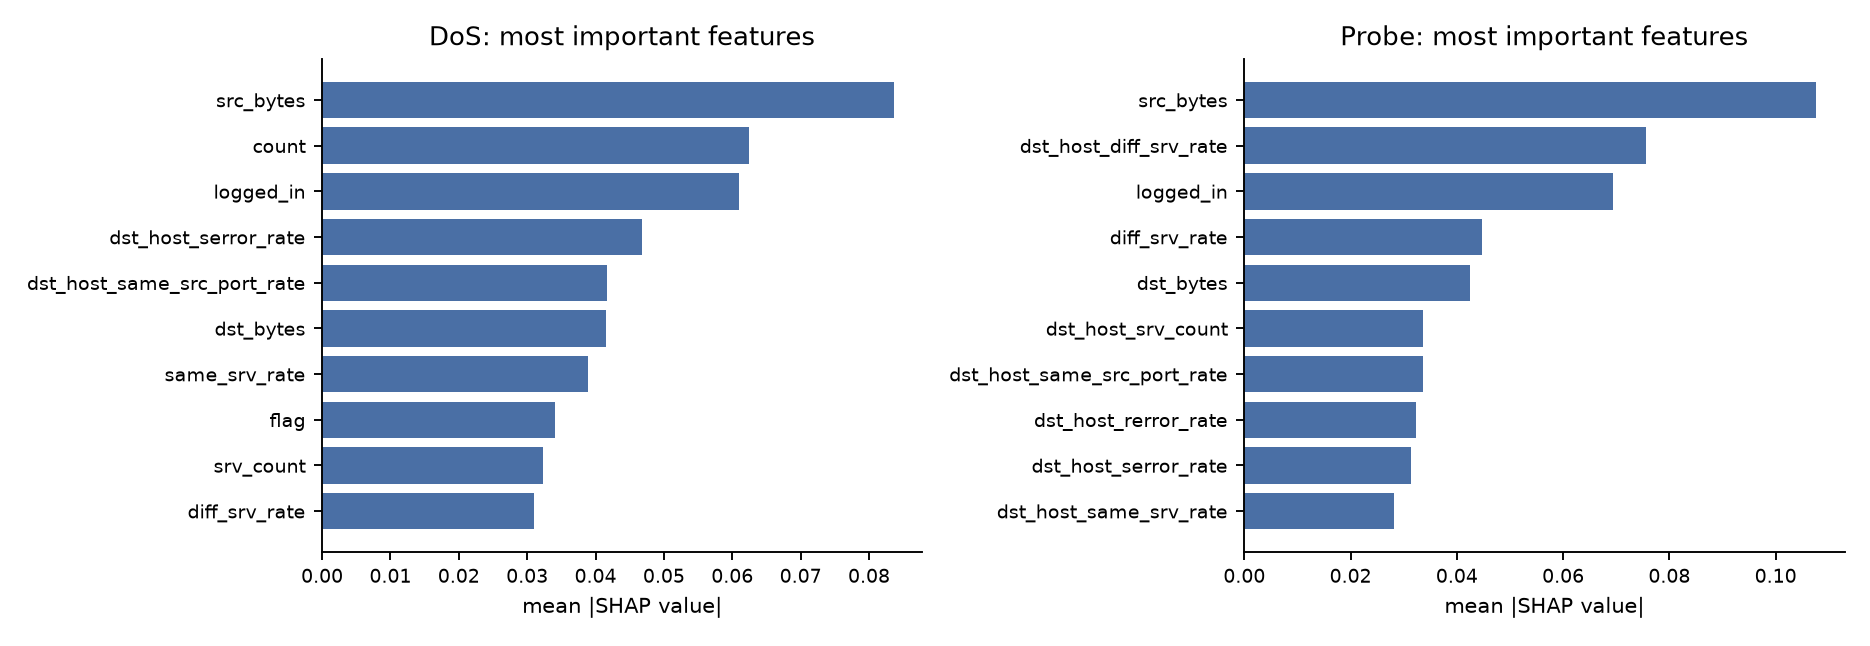
\includegraphics[width=0.93\textwidth]{../figures/shap_global.png}

\vspace{0.3em}
\raggedright\footnotesize
\begin{itemize}\itemsep2pt
  \item \textbf{DoS}: \f{src\_bytes} (almost no payload), \f{count} (many
        connections in a short window) and \f{dst\_host\_serror\_rate} (failed /
        half-open TCP handshakes) -- the classic \textbf{SYN flood} pattern.
  \item \textbf{Probe}: \f{src\_bytes}=0 combined with high
        \f{dst\_host\_diff\_srv\_rate} and \f{diff\_srv\_rate} -- empty connections
        spread over many different services, i.e.\ a \textbf{port scan}.
  \item The model relies on the same indicators an engineer would check manually.
\end{itemize}
\end{frame}

% ---------------------------------------------------------------- local DoS
\begin{frame}{Step 3: local explanation -- one blocked flow (DoS)}
\small
\begin{columns}[T]
\begin{column}{0.52\textwidth}
\centering
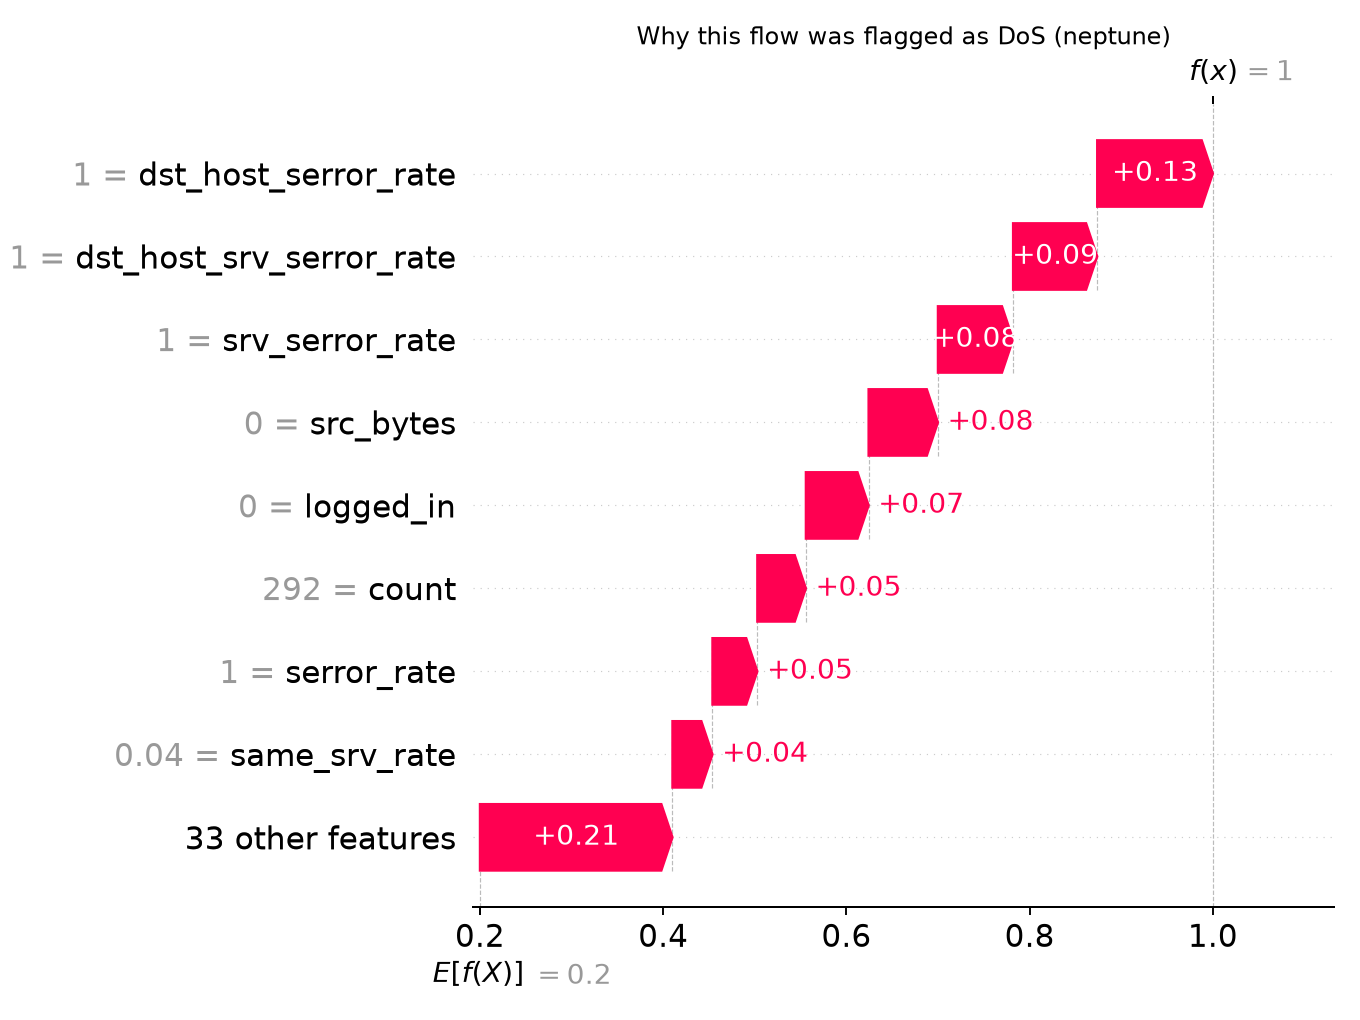
\includegraphics[width=\textwidth]{../figures/shap_local_dos.png}
\end{column}
\begin{column}{0.46\textwidth}
\vspace{1em}
A single \f{neptune} (SYN flood) flow, classified as DoS with $p=1.00$.
The bar chart starts from the average prediction $E[f(x)]=0.20$ and shows how
each feature pushed it to 1.00.

\vspace{0.8em}
Turned into a sentence an operator can read:

\vspace{0.4em}
\fbox{\parbox{0.94\linewidth}{\footnotesize
Blocked as \textbf{DoS} because the SYN error rate to this host is
\textbf{100\,\%} (\f{serror\_rate}=1), the flow carries \textbf{0 bytes}
of payload, and there were \textbf{292} connections in the time window.}}

\vspace{0.8em}
All three facts are directly verifiable in the flow record -- the engineer can
confirm or reject the verdict in seconds.
\end{column}
\end{columns}
\end{frame}

% ---------------------------------------------------------------- local Probe
\begin{frame}{Step 3: local explanation -- one blocked flow (Port scan)}
\small
\begin{columns}[T]
\begin{column}{0.52\textwidth}
\centering
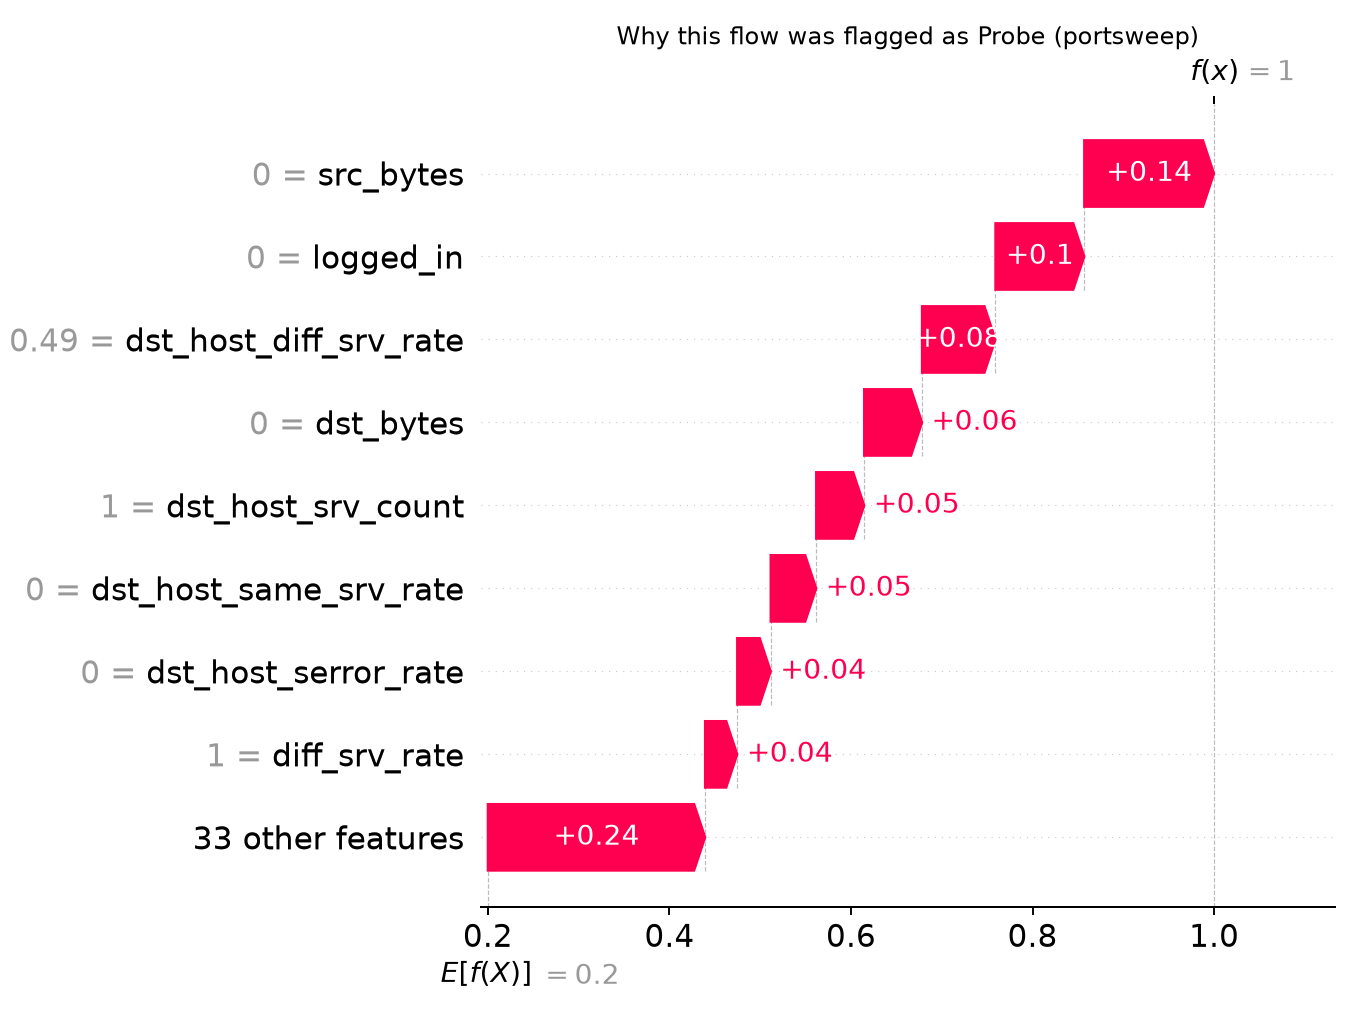
\includegraphics[width=\textwidth]{../figures/shap_local_probe.png}
\end{column}
\begin{column}{0.46\textwidth}
\vspace{1em}
A \f{portsweep} flow, classified as Probe with $p=1.00$.

\vspace{0.8em}
\fbox{\parbox{0.94\linewidth}{\footnotesize
Flagged as \textbf{Probe} because the flow sends \textbf{0 bytes}, the session
was \textbf{never logged in}, and \textbf{49\,\%} of connections to this host went
to \emph{different} services (\f{dst\_host\_diff\_srv\_rate}=0.49).}}

\vspace{0.8em}
Note how different this reason is from the DoS one: no error rates, no volume --
instead, service fan-out. The same model produces a different, attack-specific
explanation, which is exactly what makes the output useful.
\end{column}
\end{columns}
\end{frame}

% ---------------------------------------------------------------- conclusion
\begin{frame}{Conclusion}
\small
\textbf{What was done}
\begin{itemize}\itemsep2pt
  \item Trained a Random Forest IDS on NSL-KDD (74.3\,\% on the official test split).
  \item Explained it with SHAP at both levels: global feature importance per
        attack type, and per-flow waterfall plots.
\end{itemize}

\vspace{0.5em}
\textbf{What we learned}
\begin{itemize}\itemsep2pt
  \item The model's reasoning agrees with classic protocol analysis (SYN error
        rates for DoS, service fan-out for port scans), which is what makes it
        trustworthy enough to deploy.
  \item Interpretability doubles as a debugging tool (Lecture 09): the features
        SHAP highlights also explain \emph{why} R2L attacks are missed -- they leave
        no volumetric trace in a single flow.
\end{itemize}

\vspace{0.5em}
\textbf{Limitations}
\begin{itemize}\itemsep2pt
  \item NSL-KDD describes 1999-era traffic; CICIDS2017 would be the modern follow-up.
  \item TreeSHAP is exact only for tree models; a deep IDS needs the slower
        KernelSHAP or gradient-based methods.
\end{itemize}
\end{frame}

% ---------------------------------------------------------------- links
\begin{frame}{Links and references}
\footnotesize
\textbf{Code} -- one script reproduces every figure in this deck\\
\link{\repo}{github.com/Wangzx9908/ai-hw-SUMMER-2026-MRP}

\vspace{0.4em}
\textbf{Data and tools}
\begin{itemize}\itemsep1pt
  \item NSL-KDD: \link{https://www.unb.ca/cic/datasets/nsl.html}{unb.ca/cic/datasets/nsl.html}
  \item CICIDS2017: \link{https://www.unb.ca/cic/datasets/ids-2017.html}{unb.ca/cic/datasets/ids-2017.html}
  \item SHAP: \link{https://github.com/shap/shap}{github.com/shap/shap} \quad
        LIME: \link{https://github.com/marcotcr/lime}{github.com/marcotcr/lime}
  \item scikit-learn: \link{https://scikit-learn.org/}{scikit-learn.org}
  \item Interpretable ML book: \link{https://christophm.github.io/interpretable-ml-book/}{christophm.github.io/interpretable-ml-book}
\end{itemize}

\vspace{0.4em}
\textbf{References}
\begin{itemize}\itemsep1pt
  \item Lundberg \& Lee, \emph{A Unified Approach to Interpreting Model Predictions}, NeurIPS 2017.
  \item Lundberg et al., \emph{From local explanations to global understanding with explainable AI for trees}, Nature Machine Intelligence 2020.
  \item Ribeiro et al., \emph{"Why Should I Trust You?"}, KDD 2016.
  \item Sommer \& Paxson, \emph{Outside the Closed World}, IEEE S\&P 2010.
  \item Warnecke et al., \emph{Evaluating Explanation Methods for Deep Learning in Security}, IEEE EuroS\&P 2020.
  \item Wang et al., \emph{An Explainable ML Framework for Intrusion Detection Systems}, IEEE Access 2020.
  \item Tavallaee et al., \emph{A Detailed Analysis of the KDD CUP 99 Data Set}, CISDA 2009.
\end{itemize}
\end{frame}

{\setbeamertemplate{footline}{}
\begin{frame}[plain]
\vfill\centering
{\Large Thank you}\\[0.8em]
\small\link{\repo}{github.com/Wangzx9908/ai-hw-SUMMER-2026-MRP}
\vfill
\end{frame}}

\end{document}
